%!TEX root = p.tex
\section{Entity 2}
The second prototype generally received positive feedback. One of the common themes of the demos was that users liked the ability to drill down in the explorer prototype, but liked the simplicity of the entity prototype. Ultimately it seemed like we needed to add the ability to drill down further in to the newspaper data.

We decided the best way to do this, while maintaining ease of use, was to link search terms with the related terms a user clicks. That is if the user searched 'Obama' and clicked the 'Chicago' related term, then both related terms and the main plot would update with articles containing 'Obama' and 'Chicago'. We also had a breadcrumb to handle adding these additional filters. However, after a few extra filters, it wasn't uncommon for only a small number of articles to remain. In addition, this broke the free-form linking from term to term idea so we ultimately removed this feature.

Beyond this issue, there were a number of other things we needed to change after receiving feedback.

The ability to drill down to the individual article level was a common request. This actually came up in our initial interviews with journalists to understand the space as well. To address this, we added mouse over listeners on the main plot to open a dialog with appropriate article titles for the selected time.

Testers complained of unintuitive relationships between the sections of the visualization. Users were not sure whether the time slider in the main dialog affected the related term sparklines and seemed to think that the related term sparklines were the primary feature of the visualization. To address this, we placed the main sparkline above the related terms and made it larger.

A few testers wanted to see specifically related people to a given person or event. To address this we added a radio switch to see only related people, places, organizations, or all 3.

Several users were confused about how the time slider on the main sparkline related to the related term sparklines. To address this, we added a highlight to the small sparklines showing here the currently selected timespan falls. 

Several testers suggested we add instructions somewhere in the visualization. Because we did not want to take up much space with these instructions we added an information button in the top right of the visualization that has a pop up instructions dialog.

The ability to share views of the prototype also seemed very important to testers. Consequently we added a dynamic URL feature that allows sharing via URL.

The second version of the entity relation viewer, shown in \ref{explorer-1-b}, was discontinued. Though it received decent feedback, it was a difficult prototype to expand in the ways that we wanted to. In particular it was difficult to add query power, and maintain continuity between its two views. In addition, frequency comparisons did not seem as useful as we first suspected. After stopping its development, we focused on the first version of the visualization described above.

\begin{figure}[htb]
  \centerline{
    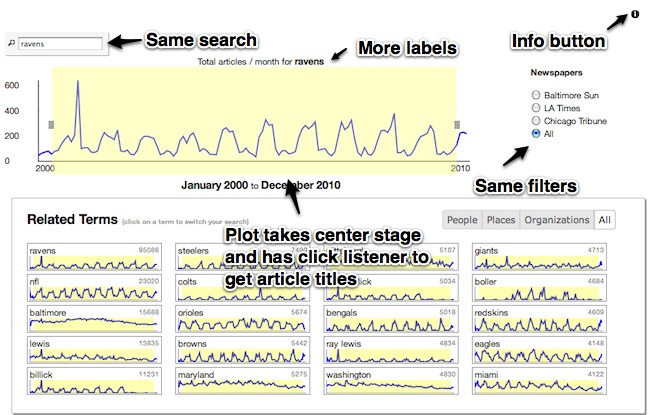
\includegraphics[scale=0.37]{figures/finalTe.jpg}
  }
  \caption{Final version of the entity explorer}
  \label{fig:explorer-1}
\end{figure}
